\documentclass[a4paper,12pt]{article}

\usepackage{fontspec} % Пакет для работы со шрифтами в XeLaTeX
\setmainfont{Liberation Serif} % Теперь эта команда сработает
\usepackage[russian]{babel}

% Математические пакеты
\usepackage{amsmath, amsfonts, amssymb}
\usepackage{geometry}
\geometry{left=3cm, right=1.5cm, top=2cm, bottom=2cm}

\usepackage{graphicx}
\usepackage{float}
\usepackage{booktabs}

\usepackage{multirow} % Обязательно добавьте этот пакет в преамбулу
\usepackage{enumerate}
\usepackage{tabularx}
\usepackage{tikz}
\usetikzlibrary{arrows.meta, calc, decorations.markings}



% Настройка стрелок для диаграмм
\tikzset{
    voltage/.style={-Stealth, thick, red},
    current/.style={-Stealth, thick, blue},
    neutral/.style={-Stealth, thick, purple},
    axis/.style={-Stealth, gray!50, thin}
}

\begin{document}

% --- ТИТУЛЬНЫЙ ЛИСТ ---
\begin{titlepage}
    \centering
    \textbf{Министерство науки и высшего образования Российской Федерации}\\
    ФЕДЕРАЛЬНОЕ ГОСУДАРСТВЕННОЕ АВТОНОМНОЕ ОБ ОБРАЗОВАТЕЛЬНОЕ\\
    УЧРЕЖДЕНИЕ ВЫСШЕГО ОБРАЗОВАНИЯ\\
    \textbf{НАЦИОНАЛЬНЫЙ ИССЛЕДОВАТЕЛЬСКИЙ УНИВЕРСИТЕТ ИТМО}\\
    \vspace{1cm}
    Факультет безопасности информационных технологий\\
    \vspace{2cm}
    Дисциплина:\\
    «Электротехника»\\
    \vspace{2cm}
    \textbf{ОТЧЕТ ПО ЛАБОРАТОРНОЙ РАБОТЕ №3}\\
    «Исследование трёхфазных электрических цепей» \\
    \vspace{3cm}
    \begin{flushright}
        \textbf{Выполнил:}\\
        Пахомов Владимир Юрьевич, студент группы N3250\\
        \vspace{0.5cm}
        \textbf{Проверил:}\\
        Кононова Мария Евгеньевна\\
    \end{flushright}
    \vfill
    Санкт-Петербург\\
    2026
\end{titlepage}

\tableofcontents
\newpage

% --- Содержание работы ---
\section{Цель работы}
Исследование свойств линейных трёхфазных цепей синусоидального тока при соединении приёмников звездой с равномерной и неравномерной нагрузкой.

\section{Исходные данные (Вариант 22)}
Параметры источника:
\begin{itemize}
    \item Амплитуда фазной ЭДС: $E_m = 63.6396$ В.
    \item Действующее значение фазной ЭДС: $E = \frac{63.6396}{\sqrt{2}} \approx 45$ В.
    \item Частота: $f = 50$ Гц.
\end{itemize}

Параметры нагрузок по типам (RL-цепи):
\begin{itemize}
    \item \textbf{z9}: $R = 56$ Ом, $L = 0.157$ Гн $\Rightarrow X_L = 2\pi f L \approx 49.32$ Ом.
    \item \textbf{z10}: $R = 50$ Ом, $L = 0.142$ Гн $\Rightarrow X_L = 2\pi f L \approx 44.61$ Ом.
    \item \textbf{z11}: $R = 45$ Ом, $L = 0.127$ Гн $\Rightarrow X_L = 2\pi f L \approx 39.90$ Ом.
\end{itemize}
Сопротивление нейтрального провода: $R_{Nn} = 0.09$ Ом.

\section{Часть I. Исследование нагрузки, соединенной по схеме «Звезда»}

\subsection{Схема эксперимента}
Схема была собрана в программной среде LTspice. Источники ЭДС соединены в «звезду», нагрузки фаз подключены к соответствующим линиям. В опытах с нейтральным проводом использовался резистор $RNn = 0.09$ Ом.

\begin{figure}[H]
    \centering
    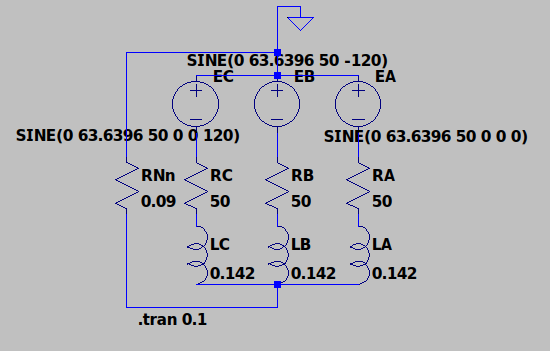
\includegraphics[width=12cm]{scheme1.png}
    \caption{Схема цепи}
\end{figure}

\subsection{Результаты измерений}
Ниже приведена таблица с данными, полученными в ходе имитационного моделирования.


\begin{table}[h!]
\centering
\caption{Таблица 3.1 — Исследование трехфазной цепи (Звезда)}
\label{tab:results_star}
\vspace{5pt}
\resizebox{\textwidth}{!}{
\begin{tabular}{|c|l|c|c|c|c|c|c|c|c|c|c|c|}
\hline
\multirow{2}{*}{№} & \multirow{2}{*}{Вид нагрузки} & \multirow{2}{*}{Тип} & $U_a$ & $U_b$ & $U_c$ & $I_a$ & $I_b$ & $I_c$ & $P_a$ & $P_b$ & $P_c$ & $I_{Nn}$ \\ \cline{4-13} 
 & & & В & В & В & А & А & А & Вт & Вт & Вт & А \\ \hline
 
\multirow{2}{*}{1} & \multirow{2}{*}{\begin{tabular}[c]{@{}l@{}}Симметричная \\ (с нулем)\end{tabular}} 
& Изм. & 45.00 & 45.00 & 45.00 & 0.671 & 0.671 & 0.671 & 22.54 & 22.54 & 22.54 & 0.00 \\ \cline{3-13} 
 & & Выч. & 45.00 & 45.00 & 45.00 & 0.672 & 0.672 & 0.672 & 22.56 & 22.56 & 22.56 & 0.00 \\ \hline

\multirow{2}{*}{2} & \multirow{2}{*}{\begin{tabular}[c]{@{}l@{}}Симметричная \\ (без нуля)\end{tabular}} 
& Изм. & 45.00 & 45.00 & 45.00 & 0.671 & 0.671 & 0.671 & 22.54 & 22.54 & 22.54 & --- \\ \cline{3-13} 
 & & Выч. & 45.00 & 45.00 & 45.00 & 0.672 & 0.672 & 0.672 & 22.56 & 22.56 & 22.56 & --- \\ \hline

\multirow{2}{*}{3} & \multirow{2}{*}{\begin{tabular}[c]{@{}l@{}}Несимметричная \\ (с нулем)\end{tabular}} 
& Изм. & 45.00 & 45.00 & 44.98 & 0.603 & 0.671 & 0.748 & 20.36 & 22.55 & 25.18 & 0.128 \\ \cline{3-13} 
 & & Выч. & 45.00 & 45.00 & 45.00 & 0.603 & 0.672 & 0.749 & 20.38 & 22.56 & 25.22 & 0.130 \\ \hline

\multirow{2}{*}{4} & \multirow{2}{*}{\begin{tabular}[c]{@{}l@{}}Несимметричная \\ (без нуля)\end{tabular}} 
& Изм. & 47.44 & 45.22 & 42.47 & 0.636 & 0.675 & 0.706 & 22.63 & 22.76 & 22.44 & --- \\ \cline{3-13} 
 & & Выч. & 47.51 & 45.30 & 42.41 & 0.637 & 0.676 & 0.706 & 22.71 & 22.84 & 22.45 & --- \\ \hline

\multirow{2}{*}{5} & \multirow{2}{*}{\begin{tabular}[c]{@{}l@{}}Обрыв фазы С \\ (с нулем)\end{tabular}} 
& Изм. & 45.01 & 44.94 & 0.00 & 0.603 & 0.670 & 0.00 & 20.37 & 22.48 & 0.00 & 0.902 \\ \cline{3-13} 
 & & Выч. & 45.00 & 45.00 & 0.00 & 0.603 & 0.672 & 0.00 & 20.38 & 22.56 & 0.00 & 0.910 \\ \hline

\multirow{2}{*}{6} & \multirow{2}{*}{\begin{tabular}[c]{@{}l@{}}Обрыв фазы С \\ (без нуля)\end{tabular}} 
& Изм. & 41.06 & 36.87 & 0.00 & 0.550 & 0.550 & 0.00 & 16.95 & 15.14 & 0.00 & --- \\ \cline{3-13} 
 & & Выч. & 41.12 & 36.93 & 0.00 & 0.551 & 0.551 & 0.00 & 17.01 & 15.19 & 0.00 & --- \\ \hline

\multirow{2}{*}{7} & \multirow{2}{*}{\begin{tabular}[c]{@{}l@{}}КЗ фазы С \\ (без нуля)\end{tabular}} 
& Изм. & 77.89 & 77.77 & 0.17 & 1.044 & 1.160 & 1.905 & 61.00 & 67.34 & 0.32 & --- \\ \cline{3-13} 
 & & Выч. & 77.94 & 77.94 & 0.00 & 1.045 & 1.163 & 2.100 & 61.12 & 67.63 & 0.00 & --- \\ \hline

\end{tabular}
}
\end{table}

\section{Расчётные формулы и расчёты}
Для аналитического расчета используется символический метод.
Комплексные сопротивления:
$\underline{Z} = R + j(2\pi f L)$.
Например, для нагрузки z10:
$\underline{Z}_{10} = 50 + j(314.16 \cdot 0.142) = 50 + j44.61 \approx 67 \cdot e^{j41.7^\circ}$ Ом.

Ток в фазе (для симметричного режима):
$\underline{I}_A = \frac{\underline{E}_A}{\underline{Z}} = \frac{45 \cdot e^{j0^\circ}}{67 \cdot e^{j41.7^\circ}} \approx 0.671 \cdot e^{-j41.7^\circ}$ А.
Экспериментальное значение $I = 0.671$ А совпадает с расчетным.

Напряжение смещения нейтрали (метод двух узлов):
$\underline{U}_{Nn} = \frac{\underline{E}_A \underline{Y}_a + \underline{E}_B \underline{Y}_b + \underline{E}_C \underline{Y}_c}{\underline{Y}_a + \underline{Y}_b + \underline{Y}_c + \underline{Y}_n}$.



\section{Векторные диаграммы}
% --- ОПЫТ 1 и 2 ---
\subsection{Опыт 1 и 2. Симметричная нагрузка}
\begin{center}
\begin{tikzpicture}[scale=1.2]
    % Оси
    \draw[axis] (-2,0) -- (2,0) node[right]{Im}; 
    \draw[axis] (0,-2) -- (0,2) node[above]{Re};
    \coordinate (O) at (0,0);
    
    % Напряжения (симметричная звезда)
    \draw[voltage] (O) -- (0,1.5) coordinate (Ua) node[right]{$U_a$};
    \draw[voltage] (Ua) -- (1.3,-0.75) coordinate (Ub) node[right]{$U_b$};
    \draw[voltage] (Ub) -- (O) node[left, pos=0.5]{$U_c$};
    
    \begin{scope}[xshift=5cm]
        \draw[axis] (-1.5,0) -- (1.5,0) node[right]{Im}; 
        \draw[axis] (0,-1.5) -- (0,1.5) node[above]{Re};
        % Токи (симметричные, сумма = 0, цепочка замыкается)
        \draw[current] (0,0) -- (0.6,0.8) coordinate (ia) node[right]{$I_a$};
        \draw[current] (ia) -- (1.1,-0.3) coordinate (ib) node[right]{$I_b$};
        \draw[current] (ib) -- (0,0) node[left, pos=0.5]{$I_c$};
    \end{scope}
\end{tikzpicture}
\end{center}

% --- ОПЫТ 3 ---
\subsection{Опыт 3. Несимметричная нагрузка с нулевым проводом}
\begin{center}
\begin{tikzpicture}[scale=1.2]
    \draw[axis] (-2,0) -- (2,0); \draw[axis] (0,-2) -- (0,2);
    \coordinate (O) at (0,0);
    \draw[voltage] (O) -- (0,1.5) coordinate (Ua) node[right]{$U_a$};
    \draw[voltage] (Ua) -- (1.3,-0.75) coordinate (Ub) node[right]{$U_b$};
    \draw[voltage] (Ub) -- (O) node[left, pos=0.5]{$U_c$};
    
    \begin{scope}[xshift=5cm]
        \draw[axis] (-1.5,0) -- (1.5,0); \draw[axis] (0,-1.5) -- (0,1.5);
        % Цепочка токов
        \draw[current] (0,0) -- (0.5,0.7) coordinate (ia) node[right]{$I_a$};
        \draw[current] (ia) -- (1.1,-0.1) coordinate (ib) node[right]{$I_b$};
        \draw[current] (ib) -- (0.4,-1.2) coordinate (ic) node[right]{$I_c$};
        % Результирующий вектор тока в нейтрали (из начала в конец цепочки)
        \draw[neutral] (0,0) -- (ic) node[left, pos=0.7]{$I_{Nn}$};
    \end{scope}
\end{tikzpicture}
\end{center}

% --- ОПЫТ 4 ---
\subsection{Опыт 4. Несимметричная нагрузка без нулевого провода}
\begin{center}
\begin{tikzpicture}[scale=1.2]
    \draw[axis] (-2,0) -- (2,0); \draw[axis] (0,-2) -- (0,2);
    \coordinate (O) at (0,0);
    % Цепочка напряжений
    \draw[voltage] (O) -- (0.2, 1.6) coordinate (Ua) node[right]{$U_a$};
    \draw[voltage] (Ua) -- (1.7, -0.6) coordinate (Ub) node[right]{$U_b$};
    \draw[voltage] (Ub) -- (0.6, -1.2) coordinate (Uc) node[below]{$U_c$};
    % Результирующий вектор -3Unn (из начала цепочки в конец)
    \draw[neutral] (O) -- (Uc) node[left, pos=0.5]{$-3U_{Nn}$};
    
    \begin{scope}[xshift=5cm]
        \draw[axis] (-1.5,0) -- (1.5,0); \draw[axis] (0,-1.5) -- (0,1.5);
        % Токи без нейтрали: сумма всегда 0 (цепь замыкается)
        \draw[current] (0,0) -- (0.6,0.9) coordinate (ia) node[right]{$I_a$};
        \draw[current] (ia) -- (1.3,-0.2) coordinate (ib) node[right]{$I_b$};
        \draw[current] (ib) -- (0,0) node[left, pos=0.5]{$I_c$};
    \end{scope}
\end{tikzpicture}
\end{center}

% --- ОПЫТ 5 ---
\subsection{Опыт 5. Обрыв фазы С с нулевым проводом}
\begin{center}
\begin{tikzpicture}[scale=1.2]
    \draw[axis] (-2,0) -- (2,0); \draw[axis] (0,-2) -- (0,2);
    \draw[voltage] (0,0) -- (0,1.5) node[right]{$U_a$};
    \draw[voltage] (0,1.5) -- (1.3,-0.75) node[right]{$U_b$};
    \node at (-0.5,-0.5) {$U_c=0$};
    
    \begin{scope}[xshift=5cm]
        \draw[axis] (-1.5,0) -- (1.5,0); \draw[axis] (0,-1.5) -- (0,1.5);
        % Цепочка токов (Ic = 0)
        \draw[current] (0,0) -- (0.5,0.7) coordinate (ia) node[right]{$I_a$};
        \draw[current] (ia) -- (1.2,-0.2) coordinate (ib) node[right]{$I_b$};
        % Результирующий вектор Inn
        \draw[neutral] (0,0) -- (ib) node[below, pos=0.5]{$I_{Nn}$};
    \end{scope}
\end{tikzpicture}
\end{center}

% --- ОПЫТ 6 ---
\subsection{Опыт 6. Обрыв фазы С без нулевого провода}
\begin{center}
\begin{tikzpicture}[scale=1.2]
    \draw[axis] (-2,0) -- (2,0); \draw[axis] (0,-2) -- (0,2);
    \coordinate (O) at (0,0);
    % Цепочка напряжений (Ua + Ub = -3Unn)
    \draw[voltage] (O) -- (0.1, 1.2) coordinate (Ua) node[right]{$U_a$};
    \draw[voltage] (Ua) -- (1.4, -0.8) coordinate (Ub) node[right]{$U_b$};
    \draw[neutral] (O) -- (Ub) node[below, pos=0.5]{$-3U_{Nn}$};
    
    \begin{scope}[xshift=5cm]
        \draw[axis] (-1.5,0) -- (1.5,0); \draw[axis] (0,-1.5) -- (0,1.5);
        % Токи: Ia = -Ib, цепочка замыкается
        \draw[current] (0,0) -- (0.7,0.7) coordinate (ia) node[right]{$I_a$};
        \draw[current] (ia) -- (0,0) node[left, pos=0.5]{$I_b$};
    \end{scope}
\end{tikzpicture}
\end{center}

% --- ОПЫТ 7 ---
\subsection{Опыт 7. Короткое замыкание фазы С}
\begin{center}
\begin{tikzpicture}[scale=1.2]
    \draw[axis] (-2,0) -- (2,0); \draw[axis] (0,-2) -- (0,2);
    \coordinate (O) at (0,0);
    % При КЗ фазы С потенциал нейтрали нагрузки совпадает с фазой С источника
    \draw[voltage] (O) -- (0, 1.8) coordinate (Ua) node[right]{$U_a$};
    \draw[voltage] (Ua) -- (1.5, -0.9) coordinate (Ub) node[right]{$U_b$};
    \draw[neutral] (O) -- (Ub) node[below, pos=0.5]{$-3U_{Nn}$}; % Uc стремится к 0
    
    \begin{scope}[xshift=5cm]
        \draw[axis] (-1.5,0) -- (1.5,0); \draw[axis] (0,-1.5) -- (0,1.5);
        % Токи: сумма 0, но векторы большие
        \draw[current] (0,0) -- (1.0,1.2) coordinate (ia) node[right]{$I_a$};
        \draw[current] (ia) -- (2.2,0.1) coordinate (ib) node[right]{$I_b$};
        \draw[current] (ib) -- (0,0) node[left, pos=0.5]{$I_c$};
    \end{scope}
\end{tikzpicture}
\end{center}

\newpage

\section{Выводы}
1. При симметричной нагрузке потенциал нейтрали нагрузки равен потенциалу нейтрали источника, ток в нейтральном проводе отсутствует. \\
2. Нейтральный провод в несимметричной системе поддерживает фазные напряжения равными. Его отсутствие при разной нагрузке приводит к значительному изменению фазных напряжений (перекосу фаз), что опасно для потребителей. \\
3. Обрыв фазы в трехпроводной системе (без нуля) превращает цепь в однофазную с последовательным соединением двух оставшихся нагрузок. \\
4. Короткое замыкание фазы без нейтрали вызывает рост напряжений на остальных фазах до линейного значения ($\approx 78$ В), что подтверждено измерениями в Опыте 7. \\




\end{document}